\setchapterpreamble[u]{\margintoc}
\glsresetall % reset glossary

\chapter{Literature review}
Introduction

This thesis is concerned with the application of optimization to the field of structural engineering. As such, knowledge of both existing optimization methods and current engineering practice is required. This chapter contains a review of current work

\section{An introduction to structural optimization}

intro on structural optimization

different families, sizing, shape and topology optimization

Numerical optimization consists of the use of algorithms to minimize or maximize a given function by varying several variables. The problem might or not be subject to constraints.

The formulation of an optimization problem is an important step that permits avoiding common conceptual errors, as confusing constraints with objective functions. If the problem formulation is wrong, the solution could fail or simply return a mathematical optimum that is not feasible engineering-wise.

The most general formulation of an optimization problem is written as:
\begin{equation}
    \begin{aligned}
    \min_{\bm{x}}         && & f(\bm{x})\\
    \textrm{by varying}   && \bm{x} &\in [l^-,l^+] \\
    \textrm{s.t.}   && c_e(\bm{x}) &= 0 \\
    && c_i(\bm{x}) &> 0, \\
    \end{aligned}
\end{equation}
where 
\begin{itemize}
    \item $ f(x) $ is the objective function to minimize
    \item $ \bm{x} $ is the vector of design variables bounded between $ l^- $ and $ l^+ $
    \item $c_e$ are the equality constraints and $c_i$ the inequality constraints.
\end{itemize}

\subsubsection{Objective Function}
In the convention of numerical optimization, the objective function $f$ is the scalar that we want to minimize. If one would instead maximize a function, then one only needs to use the inverse or the opposite of that function, in order to follow the convenction. Common objective functions in the structural design are the minimization of the weight or the structural compliance of a structure. The objective function can be modelled as an explicit function or even be the result of a highly complex computational procedure. The choice of the objective function is critical to propose a design that is feasable from the engineering point of view, regardless of the precision of the optimization scheme used.
 
Optimization problems are classified in the literature with respect to the objective function by determining how the function is linked to design variables (linear, quadratic, or generally non-linear).
 
If one would optimize a part using multiple objective functions, it is possible, but this results in a family of optimum designs with different emphasis on the various objectives. Usually, it is easier to convert these different objectives into constraints \sidecite{martins_engineering_2021}.

\subsubsection{Design Variables}
The design variables $\bm{x}$ are the parameters that the optimizer algorithm can change to minimize the objective function. Design variables could be continuous or discrete if only some distinct values are allowed (for example, only a certain size for a hole in a structural analysis). The optimization problem formulation allows for the lower and upper boundary for each design variable known in the literature as variable bounds.

\subsubsection{Constraints}
The constraints are functions used to restrict in some way the design variables. They are used to prevent the algorithm from finding a numerical minimum that is not feasible because of physical and engineering constraints. As in the case of the objective function, the constraint functions can be linear, quadratic, or generally non-linear and different algorithms must be used accordingly.
 
The constraint functions can be further classified: if the design variables are restricted to be equal to a fixed quantity, the functions are called \textit{equality constraints} ($C_e$). When instead the design variables are enforced to be greater or equal to a certain quantity the functions are called \textit{inequality constraints} ($C_i$).

\subsection{Optimizers}
Compliance minimization problems have been solved with a variety of algorithm types. There exists three
main algorithm families to perform the optimizations: optimality criteria, metaheuristic algorithms and
gradient-based strategie
The different type of approximations of the problem include among others Sequential Linear Programming
(SLP), Sequential Least Square Quadratic Programming, Augmented Lagrangian, CONvex LINearization
(CONLIN) [46] or Methods of Moving Asymptotes (MMA) [47]. Dedicated algorithms to solve the approx-
10
2.3. Strength-Based Topology Optimization
imated problems include among others the primal-dual method or interior point method. SLP consists in
solving successive linearized problem at the current iteration, whereas SLSQP uses a quadratic approximation.
The Augmented Lagrangian is an improved quadratic penalty method. CONLIN linearizes or uses an inverse
approximation, depending on the sign of the gradient. MMA consists in a monotonous approximation, which
can be controlled by the values of the asymptotes. Svanberg [48] also proposed a modification on MMA, the
Global Convergent MMA (GCMMA). The GCMMA approximation is convex and non-monotonous, which
is better suited to approach a minima without oscillations due to its non-monotonous property. Zuo et
al. [49] combined the monotonous Method of Moving Asymptotes (MMA) to initially converge faster towards
a minima for compliance minimization, and then switched to the Global Convergent MMA (GCMMA).
Strength-based topology optimization problems for isotropic materials are solved by means of gradient-based
optimizers. A variety of algorithms has been used, including among others the Augmented Lagrangian [52,
59, 61], MMA [4, 50, 51, 53, 69], CONLIN [63] or SLP [75]. In general, gradient-based algorithms are the
most extensively used in topology optimization because of their versatility, even for other constraints such
as buckling [4, 81], vibration [82] or manufacturing constraints [83, 84]. Gradient-based optimizers are also
widely used in the case of anisotropy as discussed next.

\sidecite{rojas}




\section{Ultra-lightweight structures optimization}
The introduction of new propulsion technologies (electric, LH2) aimed at reducing greenhouse gas emissions in the aeronautical sector provides an opportunity to rethink the structure design from the initial phases. The subsequent reevaluation of associated design methods has led to the exploration of structural optimization techniques. Topology optimization, in particular, offers a valuable approach to identifying optimal shapes and material distributions and allows achieving any shape within the design space instead of dealing with predefined configurations. Classical topology optimization considers the design domain as a continuum, in which each location may or may not have a material assigned to it~\cite{bendsoe_optimal_1989}. While topology optimization offers tremendous benefits in terms of weight reduction and structural efficiency, it is important to acknowledge the challenges associated with manufacturing such designs. The intricate and complex geometries generated through the optimization can pose difficulties in the fabrication process, often requiring advanced manufacturing techniques, specialized equipment, and specific constraints in the optimization \cite{zhou_progress_2002,brackett_topology_2011,liu_current_2018}. Additionally, the computational time required for generating such optimized designs, particularly for low volume fractions typical of the aerospace domain, can be significant \cite{aage_giga-voxel_2017}, impacting the overall efficiency of the design process. This remains true even with the use of adaptive meshes~\cite{salazar_de_troya_adaptive_2018, zhang_adaptive_2020}.

Even if the freedom of the design space offered by continuum meshes is high, it is known that at very low volume fractions (\eg ultralight structures), and, especially if buckling constraints and manufacturing considerations (\eg minimum length scale), are taken into account, the optimal topology is a truss-like structure~\cite{sigmund_non-optimality_2016}. Two commonly used methods for optimizing truss structures are topology optimization with explicitly defined components and \gls{tto}. 

Topology optimization methods using explicitly defined components have been developed to permit an easier interpretation of the solution, finding the optimal shape, size, and connectivity of components projected over a finite element continuum mesh. Two main feature-mapping methods applied to topology optimization have been developed\cite{wein_review_2020}, the \gls{mmc} approach \cite{guo_doing_2014,zhang_new_2017}
and the \gls{gp} approach \cite{norato_geometry_2015, zhang_geometry_2016}, later combined in a unique methodology called \gls{ggp} \cite{coniglio_generalized_2020}. Recently, the \gls{gp} approach has been used to optimize light lattice structures, proving the effectiveness of the method to provide easy-to-interpret solutions \cite{kazemi_multi-material_2020}. Nevertheless, the optimization is still based on a density field projected on a continuum mesh, that needs to be refined to correctly discretize low volume fraction structures. Additionally, truss structure design naturally depends on constraints on maximum allowable stress and buckling which are all known for being difficult to implement on topology optimization using the \gls{nand} formulation. This is principally due to the singular optima (or topologies) phenomenon~\cite{cheng_-relaxed_1997,rozvany_design-dependent_2001} and the pseudo-modes of buckling of low-density elements \cite{gao_topology_2015}.

On the other hand, \gls{tto} focuses on optimizing the topology of the truss structure itself. It involves selecting the cross-sectional areas and the connectivity of a discrete and dense mesh called ground structure, aiming to minimize weight while satisfying structural constraints~\cite{dorn_automatic_1964, fleron1964minimum}. In these classical works, the optimized structure is obtained as a subset of the initial ground structure, but multiple alternative approaches have been proposed since then, \eg starting from a very coarse ground structure that is enriched during the analysis \cite{gilbert_layout_2003}, or giving the nodes of a coarse ground structure the possibility to move, during \cite{pedersen_optimal_1973, achtziger_simultaneous_2007, descamps_lower-bound_2013}, or after the optimization, simultaneously reducing the number of active members of the solution \cite{he_rationalization_2015, lu_reducing_2023}. Recently, a hybrid method based on the projection of explicitly defined components on a discrete ground structure has been proposed, easing the interpretation of the stiffening pattern of the optimized truss \cite{savine_component-based_2021}.

In the early works, the \gls{tto} problem was formulated in terms of member forces \cite{dorn_automatic_1964, hemp_optimum_1973} with plastic material modelization, ignoring the kinematic compatibility to obtain a \gls{lp} problem. Formulated using the \gls{sand} approach, the equations of structural mechanics of the problem are imposed as constraints of the optimization and, contrary to \gls{nand} approaches, are not explicitly solved. Formulated that way, it is trivial to add maximum stress constraints compared to an equivalent \gls{nand} formulation. However, the \gls{sand} formulation with plastic material modelization only correctly predicts the mechanical behavior of statically determinate structures or mechanisms \cite{kirsch_optimal_1989, rozvany_layout_1995}. Moreover, adding local buckling constraints to the optimization formulation is fundamental, as ultralight truss structures are often dominated by this mode of failure \cite{sigmund_non-optimality_2016}. Multiple works in the field of truss structure optimization have focused on addressing these two crucial challenges \cite{kirsch_optimal_1980,cheng_aspects_1995,achtziger_local_1999}.

Ultralight trusses are a good design candidate for the design of innovative aerostructures thanks to their superior aeroelastic properties and stiffness-to-weight ratio \cite{cramer_elastic_2019}. These structures represent a natural application case for the discussed optimization formulations. \cite{opgenoord_aeroelastic_2018, opgenoord_design_2019} proposed a two-step sequential optimization algorithm to reduce the weight of a truss wing. Firstly, a ground structure with different nodal densities based on the stress field of the structure is generated and secondly, the cross-sectional areas are found using a sizing optimization algorithm that takes into account stress, local buckling, and aeroelastic constraints. \cite{shahabsafa_novel_2018} decided, instead, to tackle all the difficulties of the problem using a set of discrete cross-sectional areas and a sizing \gls{milo} algorithm. The algorithm is validated on a 315-bars wingbox ground structure, based on the \gls{crm}. In these studies, the adoption of a sizing optimization algorithm simplifies the numerical complexities associated with the problem. However, by solely focusing on modifying the component sizes, the opportunity to optimize the overall truss topology is missed, limiting the potential for further weight savings.

\subsection{Density based topology optimization}

\paragraph{Minimum compliance formulation}
\begin{marginfigure}
    \centering
    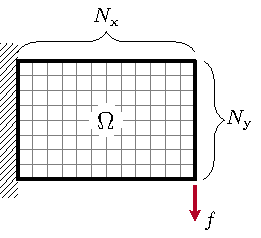
\includegraphics{figures/03_comparison_TO_TTO/01_contin_mesh/c_mesh.pdf}
    \caption{The domain $\Omega$ is discretized using $N_\text{e}=N_\text{x} N_\text{y}$ continuous 4-nodes elements.}
    \label{fig:03_mesh_c}
\end{marginfigure}
Let $\Omega \in \mathbb{R}^2$ be a rectangular domain in of dimensions $X$ and $Y$, containing respectively $N_\text{x}$ and $N_\text{y}$ linear 4-nodes elements, for a total of $N_\text{e}=N_\text{x} N_\text{y}$ elements and $M$ nodes (see \figref{fig:03_mesh_c}). The objective of the optimization is the minimization of the compliance $C$ of the structure, equivalent to finding the structure with the least possible nodal displacement with respect to a defined set of boundary conditions. The Problem $\mathbb{T}_0$ is stated in terms of the design variables $\vect{\rho}$ as follows:
\begin{equation}
    \begin{aligned}
    \min_{\vect{\rho}}         && C &= \sum_{i} \vect{u}_{e,i}^T \matr{K}_{e,i} \vect{u}_{e,i}=\vect{f}^T\vect{u}&& \forall i \in [0,\dots,N_\text{e}]                         \\
    \textrm{s.t.}   && & \frac{\sum_{i} \left(\rhophys_i v_i \right) / V_0}{V_\text{p}} - 1 \leq 0 && \forall i \in [0,\dots,N_\text{e}] \\
    && \matr{K}\vect{u} &= \vect{f} &&\\
    && 0 &\leq \rho_i \leq 1. && \forall i \in [0,\dots,N_\text{e}] \\
    \end{aligned}
    \tag{$\mathbb{T}_0$}
    \label{eq:03_prob-comp}
\end{equation}
The design variables $\vect{\rho}$ are defined for every element of the structure as $\vect{\rho} = [\rho_1, \rho_2, \ldots,\rho_{Ne}]^T$, with $\rho_i \in [0,1], \; \forall i \in [0,\dots,N_\text{e}]$. The physical densities $\vect{\rhophys}$ are related to design variables through density filtering and threshold projection~\sidecite{wang_projection_2011}, as explained later in the document. $V_\text{p}$ is the prescribed volume fraction that acts as the constraint of the minimization problem, while $v_i$ represents the area of the $i$-th element and $V_0$ is the total area of the domain $\Omega$. $\matr{K}\vect{u} = \vect{f}$ is the state equation of the problem and defines the elastic response of the structure to an external nodal load $\vect{f}=[f_1, f_2, \ldots,f_{2M}]^T$. The global stiffness matrix $\matr{K}$ is assembled from the element stiffness matrix $\matr{K} = \sum_{i \in \Omega} \matr{K}_{e,i}$ and $\matr{K}_{e,i} = E_i \matr{K}_{e,0}$ where $\matr{K}_{e,0}$ represents the element stiffness matrix relative to the chosen type of element (linear or quadratic) and $E_i(\rhophys_i)$ the Young's modulus of the $i$-th element. 

The material scheme used to interpolate between void and full material is the well-known \gls{simp}~\sideciteonce{bendsoe_optimal_1989,bendsoe_material_1999} approach. It is governed by the equation:
\begin{equation}
    E_i(\rhophys_i) = E_{\textrm{min}} + \rhophys_i^p(E_0-E_{\textrm{min}}),
    \label{eq:03_simp}
\end{equation}
where the parameter $p$ penalizes the intermediate densities and pushes the result to a black-and-white result. $E_0$ is the Young's modulus of the dense material and $E_{\textrm{min}}$ is a small value used to avoid the global stiffness matrix $\matr{K}$ from being singular when $\rhophys_i=0$. 

In this study we set these parameters to $E_0 = 1$, and $E_{\textrm{min}} = 10^{-9}$. The value of the penalization parameter $p$ is selected as $p=3$ because in that way the intermediate densities respect the \gls{hs} bounds~\sideciteonce{hashin_variational_1963,bendsoe_material_1999}. These relationships describe the boundaries of attainable isotropic material characteristics when dealing with composites (materials with microscopic structures) using two specified, linearly elastic, isotropic materials (in our case the solid and the empty phases).
\paragraph{Spatial filtering and projection}
Multiple approaches have been developed to solve the problems linked to mesh discretization, such as mesh dependence or the checkerboard problem~\sidecite{diaz_checkerboard_1995}. Filtering the sensitivity information of the optimization problem proved to be an effective approach to guarantee independence from mesh resolution~\sidecite{sigmund_design_1994,
sigmund_design_1997}. In the present research, we decided instead to directly filter the density field $\vect{\rho}$ using the 2D convolution operator~\sidecite{sigmund_morphology-based_2007}. The weight function $w$ (or kernel) of the convolution is defined as:
\begin{equation}
    w(d_j) = R - d_j, \quad j \in \mathbb{N}_{i,R}
\end{equation} 
where $\mathbb{N}_{i,R}$ represent the set of elements lying within a circle of radius $R$ centered on the $i$-th element and $d_j$ is the distance of the $j$-th element to the center of the filter (see \figref{fig:03_ker}).
\begin{marginfigure}
    \centering
    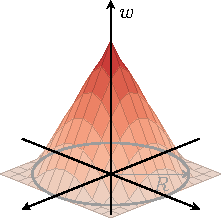
\includegraphics{figures/03_comparison_TO_TTO/02_circ_filter/filt_cir.pdf}
    \caption{Kernel of the 2D convolution operator.}
    \label{fig:03_ker}
\end{marginfigure} 
The filtered values of the design variable are calculated as:
\begin{equation}
    \rhofil_i = \frac{\sum_{j \in \mathbb{N}_{i,R}} w(d_j)v_j\rho_j}{\sum_{j \in \mathbb{N}_{i,R}} w(d_j)v_j}.
    \label{eq:03_rhofil}
\end{equation}
As the filtering phase produces a large number of gray elements, a smooth projection technique based on the \textit{tanh} function is implemented~\sidecite{wang_projection_2011}:
\begin{equation}
    \rhophys_j = \frac{\tanh(\beta\eta)+\tanh(\beta(\rhofil_j - \eta))}{\tanh(\beta\eta)+\tanh(\beta(1 - \eta))},
    \label{eq:03_proj}
\end{equation}
where $\beta$ is a parameter that defines the slope of this approximation function: the larger the value of $\beta$, the less intermediate elements are present in the structure topology. $\eta$ is the threshold value of the projection. Using \eqref{eq:03_proj} is not volume conservative for all values of $\eta$, and to stay conservative we use a volume-increasing filter~\sidecite{ferrari_new_2020}. The value of $\eta = 0.4$ is then chosen.

The derivative of the filtered density $\vect{\rhofil}$ with respect to the design variable $\vect{\rho}$ is written deriving \eqref{eq:03_rhofil}:
\begin{equation}
    \derfrac{\rhofil_i}{\rho_j} = \frac{w(d_j)v_j}{\sum_{j \in \mathbb{N}_{i,R}} w(d_j)v_j}.
    \label{eq:03_sens_filt}
\end{equation}
The sensitivity of the physical densities $\bm{\rhophys}$ with respect to the filtered $\bm{\rhofil}$ can be written as:
\begin{equation}
    \derfrac{\rhophys_j}{\rhofil_j} = \beta \frac{1-\tanh^2(\beta(\rhofil_j-\eta))}{\tanh(\beta\eta)+\tanh(\beta(1 - \eta))}.
    \label{eq:03_sens_proj}
\end{equation}
Using the chain rule it is possible to write:
\begin{equation}
    \label{eq:03_chain}
    \derfrac{h}{\rho_i} = \sum_{j \in \mathbb{N}_{i,R}} \derfrac{f}{\rhophys_j} \derfrac{\rhophys_j}{\rhofil_j} \derfrac{\rhofil_j}{\rho_i},
\end{equation}
where $h$ represents a generic function.

density methods
compliance formulation
simp ramp HS and continuation scheme
filter

accenna level set, ma tanto no serve per questa tesi

\subsection{Feature-Mapping topology optimization}
coniglio guarda che fa

\subsection{Truss topology optimization}
\paragraph{Classical Michell structures} \label{sec:03_michell}
The characteristics of these structures are described by some simple criteria that date to the end of the 19th and the beginning of the 20th century. When a structure is statically determinate — \ie the structure is not a mechanism, and it is not over-constrained by the supports — the Maxwell theorem~\sidecite{maxwell_ireciprocal_1870} states that:
\begin{equation} \label{eq:03_maxwell-th}
    \sum_{\forall i | q_i>0}\ell_iq_i + \sum_{\forall i | q_i<0}\ell_iq_i = \textrm{const.}
\end{equation}
where $\ell_i$ and $q_i$ represent the length and the axial force of the $i$-th member, respectively. The constant value at the right of~\eqref{eq:03_maxwell-th} depends on the nature of the boundary conditions and the material used. The Maxwell theorem dictates that any increment in compression forces must be counterbalanced by an equivalent increase in tension forces when the structure remains topologically unchanged. So for statically determinate structures the structure layout is not influenced by the ratio between $\sigma_\text{c}$ and $\sigma_\text{t}$, Young's modulus $E$ of the material, nor the force magnitude.

Starting from Maxwell's findings, Michell theorized two further criteria for optimal truss structures~\sidecite{michell_limits_1904} valid when the maximum allowable stress is equal in tension and compression ($\sigma_\text{t} = \sigma_\text{c}$) and when the supports of the structure are statically determinate. The first one states that all the members of an optimal structure should present internal stress equal in magnitude to the maximum allowable value of the material -- \ie the structure is \textit{fully stressed}. The second criterion asserts that the strain of all the members of the structure should be equal and there should be no other point having a strain higher than this value. As formulated, these two criteria are known as the Michell criteria. The second criterion was later generalized by Hemp~\sidecite{hemp_optimum_1973} as:
\begin{equation} \label{eq:03_hemp}
    -\frac{1}{\sigma_\text{c}}\leq \varepsilon \leq \frac{1}{\sigma_\text{t}}.
\end{equation}
Compared to the second Michell criterion, \eqref{eq:03_hemp} permits to correct identification of the minimum volume structure even when different strength values for compression and tension and different support types are taken. These criteria are known as the Michell-Hemp criteria.

\paragraph{Plastic material formulation}
The rigid-plastic formulation characterizes the material as entirely rigid up to the point of reaching the yield stress, denoted as $\sigma_y$, and subsequently assumes a constant stress level of $\sigma_y$ once that threshold is exceeded. This formulation is a clear consequence of the application of the Michell-Hemp criteria and has thus been used in the very first work of layout optimization (also known as \gls{tto})~\sidecite{dorn_automatic_1964,chan_optimum_1964,hemp_optimum_1973}. 

\paragraph{The ground structure approach}
The ground structure is a framework composed of various structural members that connect specified points or nodes in two- or three-dimensional space (see \figref{fig:03_mesh_d}). These members can take the form of beams, columns, wires, or bars elements, depending on the specific structural requirements. In this thesis, we will deal with trusses, and so the chosen element is the bar. Since the nodes within the ground structure are considered pin-joints, all straight members exclusively face either tension or compression loads. 
\begin{marginfigure}
    \centering
    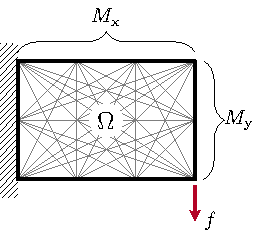
\includegraphics{figures/03_comparison_TO_TTO/04_disc_mesh/d_mesh.pdf}
    \caption{The domain $\Omega$ is discretized using a set of straight members connecting a set of nodes. This framework is known as the ground structure.}
    \label{fig:03_mesh_d}
\end{marginfigure}

Depending on how the connectivity of the grid of nodes is, we can experience very different ground structures. In a fully connected ground structure, every node within the system is linked to every other node, resulting in a dense and redundant structural configuration. The number of bars $N_{\text{el}}$ of a fully connected ground structure can be determined using the following formula:
\begin{equation}
    N_{\text{el}} = \frac{M \cdot (M-1)}{2},
\end{equation}
where $M$ represents the number of nodes of the structure.

In classic works, the ground structure is used as the start of the optimization, where the optimized structure is obtained as a subset of the initial ground structure, but multiple alternative approaches have been proposed since then, \eg starting from a very coarse ground structure that is enriched during the analysis~\sidecite{gilbert_layout_2003}, or giving the nodes of a coarse ground structure the possibility to move, during~\sidecite{pedersen_optimal_1973, achtziger_simultaneous_2007, descamps_lower-bound_2013}, or after the optimization, simultaneously reducing the number of active members of the solution~\sidecite{he_rationalization_2015, lu_reducing_2023}.

\section{Cellular structures optimization}
why modular, which are the advantages

define modules and subdomains

intro there are different type of approach that we could use, full scale and multiscale

intro multiscale.

numerical homogenization
Multi-Scale Approaches
A multi-scale approach is based on a microstructure in a representative elementary volume (REV). The
macroscopic stiffness tensor of the REV [QH ] is obtained by homogenization of the stiffness properties of its
constituents. Several homogenization methods can be used such as strain energy methods [86] or asymptotic
methods [87]. An example of asymptotic homogenization is given by Equation 2.11. chi0(ij)
e are the test strains
as presented in Figure 2.8 and chi(ij)
e the corresponding response strains. The macroscopic stiffness properties
are then used in the later process to set up the FEM analysis in topology optimization. Even when using a
mixture of only isotropic material and void at the microscale, depending on the layout of the microstructure,
an anisotropic macroscopic stiffness can be obtained

intro full scale

the problem on the number of subsections needed to correctly foresee the mechanical behaviour

In the past, the properties of materials have been altered by varying the chemical composition, microstructure and production process. Another possible way to further modify the material properties is to tailor the spatial configuration of solids and voids of the material. The so-called architectured materials are now becoming a hot topic in the research field, also thanks to the recent advances in additive manufacturing.

Extensively present in nature (e.g., bone-microstructure or birds beak), their research interest came thanks to the observation that the stiffness of optimal structures spans multiple scales \sidecite{kohn_optimal_1986,allaire_optimal_1999}. In addition to that, Fleck observed that \sidecite{fleck_micro-architectured_2010}~``\textit{one reason for such structural hierarchy in engineering structures is to increase buckling strength: recall that the buckling strength scales with any representative strut length $l$ according to $l^{-2}$, and so the finer the length scale, the higher the buckling strength}.''

If we observe the Ashby material chart \sidecite{ashby_materials_1999} of the yield strength plotted versus their density (Fig.~\ref{fig:ash1}), we can see plenty of empty spaces. Besides some unattainable spaces described by the Hashin-Shtrikman (HS) bounds \sidenote[$\dagger$]{The Hashin-Shtrikman bounds are the tightest bounds possible from the range of composite moduli for a two-phase material. In lattices, usually, the second material is substituted with void.}\sidecite{hashin_variational_1963}, these empty spaces can be filled by lattices (see Fig.~\ref{fig:ash2}), extending the property space of actual materials.

Lattices can be classified as open- or closed-wall. Even if a closed-wall lattice would result in a more stiff structure, the interest of an open-cell is well described by Sigmund et al. \sidecite{sigmund_non-optimality_2016}: ``\textit{we emphasize that the outcome of minimum compliance-type continuum topology optimization studies should always be of sheet type unless other constraints [...] that favour Michell-like structures have been explicitly stated}'', where the possible constraints are:
\begin{itemize}
    \item \textbf{Structural and Microstructural stability}: The load for initiating buckling of a slender strut is much higher than that of a comparable plate with the same mass \sidecite{deshpande_foam_2001}. An open-cell structure, thus, is less prone to buckle compared to a closed-cell.
    \item \textbf{Porosity}: A porous open-wall cell permits a flow to pass through. This property enables the use of lattice as heat exchangers or to mimic the bone microstructure.
    \item \textbf{Manufacturing}: very thin walls are extremely difficult to manufacture. An open-cell design, while being far from easy to manufacture, is then preferable from a manufacturing standpoint. 
    \item \textbf{Transparency}: The possibility to view through the structure can be beneficial for example for reparation and health monitoring.
    \item \textbf{Elegance/aesthetic}: According to Sigmund et al.~\cite{sigmund_non-optimality_2016} an open-cell design is a Michell-like structure, that are \textit{inarguably beautiful} and \textit{look elegant and efficient}.
\end{itemize}

In function of the size of the repeating cell, is it possible to distinguish a lattice material or a lattice structure, with the former having no scale separation between the cell and the macro-structure. Even if there is no clear threshold between the two, this definition will be very useful when we will talk about lattices optimization.

The relative density of the lattice is defined as:
\begin{equation}
    \bar{\rho} = \frac{\rho_l}{\rho}
\end{equation}
where $\rho_l$ and $\rho$ represent the density of the lattice and of the dense material, respectively \sidecite{ashby_properties_2006}.

We can define a stretching-dominated structure as a lattice whose constitutive struts faces only tension and compression loads. The nodal stiffness does not take part in the structural stiffness and the truss collapses by stretching of the struts. According to Desphande et al.~\sidecite{deshpande_foam_2001} on a stretching-dominated truss ``\textit{freezing the joints of the triangulated structure has virtually no effect on the macroscopic stiffness or strength; although the struts bend, the frame is still stretching-dominated and the collapse load is dictated mainly by the axial strength of the struts.}'. An open-cell structure can thus be treated as a connected set of pin-jointed struts if it is stretching-dominated.

A stretching-dominated structure is typically 10 times more stiff and 3 times more strong than a bending-dominated structure at $\bar{\rho} = 0.1$ (see Fig.~\ref{fig:str-bend}) \cite{deshpande_foam_2001}. However, in compression they present a softening post-yield response due to buckling of struts, making them non-interesting for energy absorption tasks. On the other side, bending-dominated lattices absorb more energy due to their plateau-like response.

% \begin{marginfigure}
%     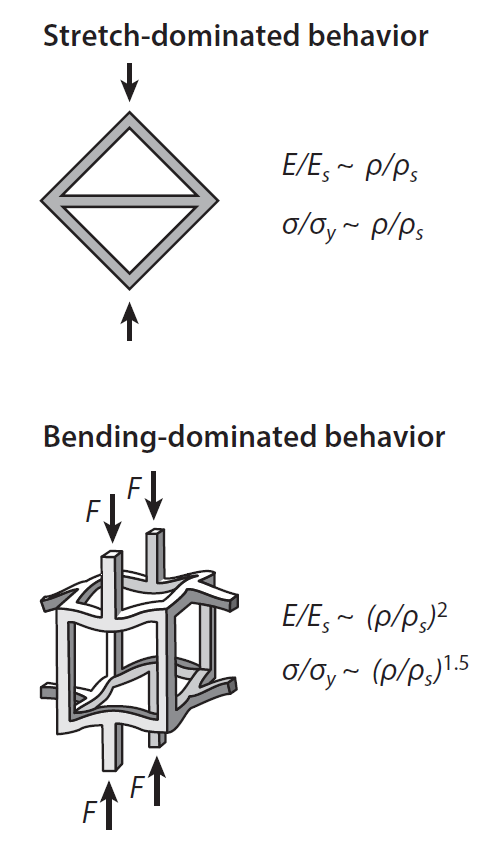
\includegraphics[width=\textwidth]{figures/stretc-bend.png}
%     \caption{A stretch-dominated and a bending-dominated cell. Bending-dominated structure act as a mechanism when the joints are pin. The scaling laws are different for the two structure families\cite{schaedler_architected_2016}.}
%     \label{fig:str-bend}
% \end{marginfigure}

Lattices structures and materials have various promising application as:
\begin{itemize}
    \item Lattice structures and materials shows notable energy absorbing properties, even more if designed as bending-dominated \sidecite{evans_concepts_2010,schaedler_designing_2014,ozdemir_energy_2016}.
    \item As a direct consequence, lattice structures are set to be the possible new design scheme for aerodynamic structures. They show remarkable aeroelastic properties \sidecite{opgenoord_aeroelastic_2018,cramer_elastic_2019}.
    \item Lattices proved to be really interesting candidates to build scaffolds \sidecite{hutmacher_scaffolds_2000,mota_additive_2015,nikolova_recent_2019}.
    \item Lattice materials present very good heat exchanger properties. This is due to their high surface-to-volume ratio and the turbulent mixing flow they create when a fluid pass through \sidecite{lu_heat_1998,wadley_thermal_2007}.
\end{itemize}

% \begin{marginfigure}
%         
\includegraphics[width=\linewidth]{figures/Loch_Ness_Wellington_(226386778).jpg}
%         \caption{Vickers Wellingtons — bombers that were used during World War II — continued functioning even with the huge amount of damages thanks to lattice fuselage. When one of the ribs was damages the load were reallocated to the other, and the structure showed still functional.}
%         \label{fig:vick}
% \end{marginfigure}
Other interesting properties of lattice structures and materials are:
\begin{itemize}
    \item Cellular structures can be designed to be reversibly assembled. This concept paves the way to rapid assembly and easy-to-repair structures. Various approach have been proposed, as using fasteners \sidecite{cheung_reversibly_2013,jenett_digital_2017,cramer_elastic_2019} or snap-fit joints \sidecite{dong_mechanical_2015}
    \item     
    
    Lattice structures are naturally damage-tolerant structures \sidecite{stolpe_fail-safe_2019,wu_topology_2021}. In a skin-lattice design, the skin is not load-bearing, and skin damage will not cause a progressive failure of the structure. Moreover, in case of rib damage, the damaged rib will be excluded from the load without any harm to the whole structure (see Fig.~\ref{fig:vick}).
    \item They open the way for an extensive use of robotization for the manufacture \sidecite{hunt_wraptor_2019} and the assembly phases \sidecite{gershenfeld_macrofabrication_2015,jenett_bill-e_2017,costa_algorithmic_2020,niehs_recognition_2020}.
\end{itemize}

This field is now getting more and more interesting, especially in the aerospace field, as we can see by the recent applications by NASA project MADCAT \sidecite{cramer_elastic_2019} and Opgenoord PhD thesis \sidecite{opgenoord_transonic_2018}.

\subsection{Multi-scale structures optimization}

\subsection{Full-scale structures optimization}

Although the aforementioned methods are able to design a structure consisting of a simple module repeated several times in the global domain, they suffer from a common limitation. Namely, the designs converge towards solutions with compromised structural performance (Huang and Xie 2008; Zhang and Sun 2006). The cause lies within the topological periodicity. The topology of the module is influenced most by the region with the highest compliance. The resulting module design is used at different locations in the structure, therefore not leading to the most optimal solution for these regions (Tugilimana et al. 2019). This shortcoming can be addressed by two approaches: (i) by defining additional module properties as design variables or (ii) by allowing more modules within the structure. Both approaches extend the solution space. The first approach, extending the solution space, was considered by allowing for rotation of a module. Allowing for rotations resulted in improved structural performance because rotation of the modules modifies the material distribution in the structure locally (Tugilimana et al. 2017). Also, in a 2D continuum setting, the one-to-one mapping of a module unit to the global domain is extended by by allowing the module unit to resize (Stromberg et al. 2011).  \sidecite{bakker_simultaneous_2021}